\documentclass[11pt,a4paper]{article}
\usepackage{amssymb} %mathbb
\usepackage{amsmath} %align
\usepackage{graphicx} %jpg
\usepackage{hyperref}
\usepackage{cancel}
\usepackage{tikz-cd}
\usepackage[top=1.0cm,bottom=1.3cm,left=1.0cm,right=1.0cm]{geometry}
\usepackage{array,bm}
\newcolumntype{C}{>{$}c<{$}}
\renewcommand{\arraystretch}{1.2}
\newenvironment{myenum}
{ \begin{enumerate}
    \setlength{\itemsep}{0pt}
    \setlength{\parskip}{0pt}
    \setlength{\parsep}{0pt}     }
{ \end{enumerate}                  }
\begin{document}

	\small

		Whole mathematics | without categories | is context free. By Vinicius Claudino Ferraz.

		\vspace{3mm}

		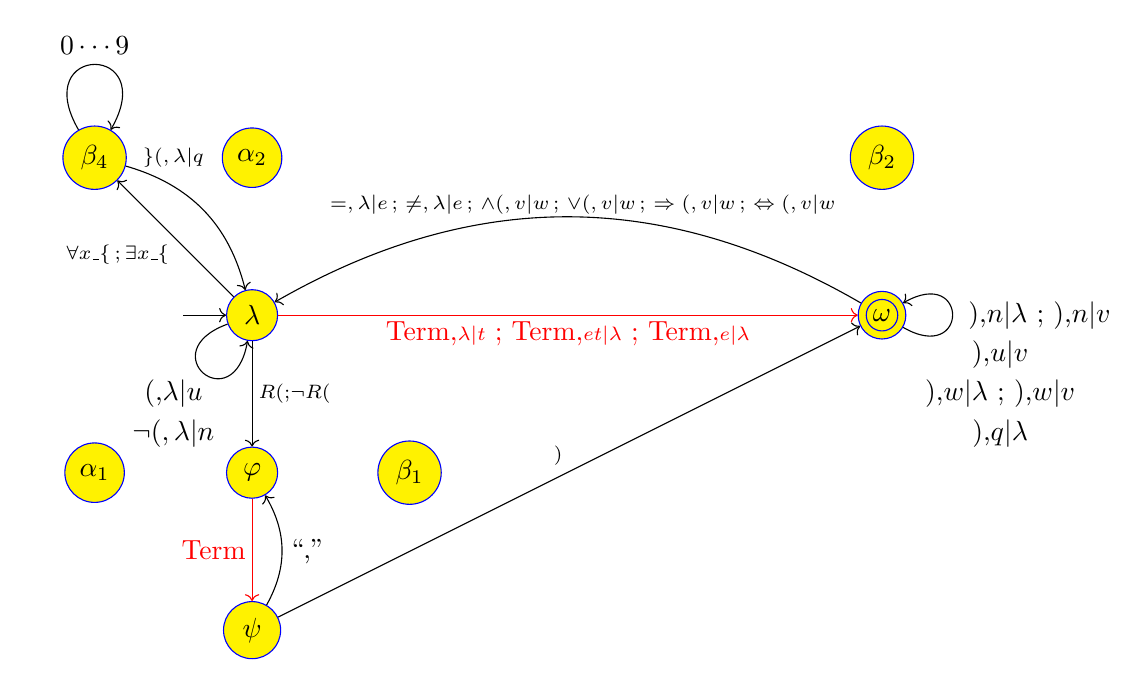
\begin{tikzpicture}
		\node (nada) at (2,0) { };
		\node[draw=blue, circle, fill=yellow] (lambda) at (3,0) {$\lambda$};
		\node (lambdalinha1) at (2,-1) {(,$\lambda|u$};
		\node (lambdalinha2) at (2,-1.5) {$\neg(,\lambda|n$};
		\node[font=\scriptsize] (lambdalinha3) at (2, 2) {$\}(,\lambda|q$};
		\draw[->] (lambda) to [in=260,out=200, loop, " "] node { } (lambda);
		\node[font=\scriptsize] (etalinha2) at (7.2, 1.4) {$=,\lambda|e\,;\,\ne,\lambda|e\,;\,\wedge(, v|w\,;\,\vee(, v|w\,;\,\Rightarrow(, v|w\,;\,\Leftrightarrow(, v|w$};
		\node[draw=blue, circle, fill=yellow] (omega) at (11,0) {$\omega$};
		\node (omegalinha1) at (13, 0) {),$n|\lambda$ ; ),$n|v$};
		\node (omegalinha2) at (12.5, -0.5) {),$u|v$};
		\node (omegalinha3) at (12.5, -1) {),$w|\lambda$ ; ),$w|v$};
		\node (omegalinha3) at (12.5, -1.5) {),$q|\lambda$};
		\draw[blue] (11,0) circle (0.2);
		\draw[->] (omega) to [in=30,out=330, loop, " "] node { } (omega);
		\node[draw=blue, circle, fill=yellow] (varphi) at (3,-2) {$\varphi$};
		\node[draw=blue, circle, fill=yellow] (alpha1) at (1,-2) {$\alpha_1$};
		\node[draw=blue, circle, fill=yellow] (c1) at (5,-2) {$\beta_1$};
		\node[draw=blue, circle, fill=yellow] (psi) at (3,-4) {$\psi$};
		\node (psilinha) at (3.7, -3) {``,"};
		\node[draw=blue, circle, fill=yellow] (c4) at (1,2) {$\beta_4$};
		\node[draw=blue, circle, fill=yellow] (alpha2) at (3,2) {$\alpha_2$};
		\node[draw=blue, circle, fill=yellow] (c2) at (11,2) {$\beta_2$};
		\draw[->] (c4) to [in=60,out=120, loop, "$0\cdots 9$"] node { } (c4);
		\draw[->, bend right] (psi) to node { } (varphi);
		\draw[->, bend left] (c4) to node { } (lambda);
		\draw[->, bend right] (omega) to node { } (lambda);
		\path[commutative diagrams/.cd, every arrow, every label]
		(nada) edge node { } (lambda)
		(lambda) edge[red] node[swap] {Term,$\lambda|t$ ; Term,$et|\lambda$ ; Term,$e|\lambda$} (omega) edge node {$R( ; \neg R($} (varphi) edge node {$\forall x\_\{\,;\,\exists x \_\{$} (c4)
		(varphi) edge[red] node[swap] {Term} (psi)
		(psi) edge node {$)$} (omega);
		\end{tikzpicture}

		\vspace{3mm}

		$F \rightarrow$ Term $ZB$

		$B \rightarrow$ Term

		$B \rightarrow$ Term $ZB$

		$R \rightarrow ``R"\_\{N\}(P)$

		$R \rightarrow\,\neg ``R"\_\{N\}(P)$

		$P \rightarrow$ Term

		$P \rightarrow P, P$

		$\lambda \rightarrow F$

		$\lambda \rightarrow GYG$

		$\lambda \rightarrow R$

		$G \rightarrow (F)$

		$G \rightarrow GYG$

		$G \rightarrow (GYG)$

		$G \rightarrow R$

		$G \rightarrow\,\neg (_nF)_n$

		$F \rightarrow Q x\_\{N\} (_nF)_n$

		$F \rightarrow Q x\_\{N\} \neg(_nF)_n$

		$F \rightarrow Q x\_\{N\} R$

		$Q \rightarrow \forall\,|\,\exists$

		$N \rightarrow NN$

		$N \rightarrow 0|1|2|3|4|5|6|7|8|9$

		$Y \rightarrow \wedge|\vee|\Rightarrow|\Leftrightarrow$

		$Z \rightarrow\,=|\ne$

		\vspace{3mm}

		Now we're going to define a Term.

		\vspace{3mm}

		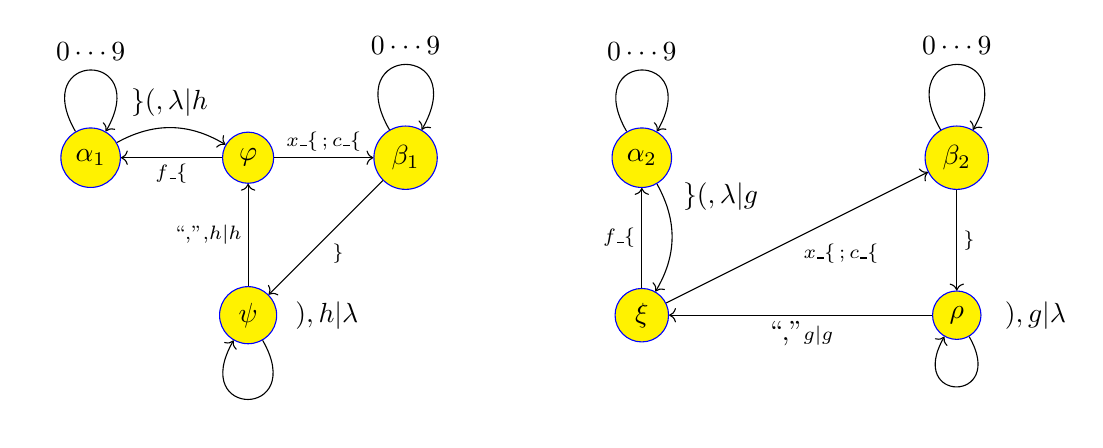
\begin{tikzpicture}
		\node[draw=blue, circle, fill=yellow] (alpha) at (0,-2) {$\alpha_1$};
		\node (alphalinha) at (1, -1.3) {$\}(,\lambda|h$};
		\draw[->] (alpha) to [in=60,out=120, loop, "$0\cdots9$"] node { } (alpha);
		\node[draw=blue, circle, fill=yellow] (varphi) at (2,-2) {$\varphi$};
		\node[draw=blue, circle, fill=yellow] (c) at (4,-2) {$\beta_1$};
		\draw[->] (c) to [in=60,out=120, loop, "$0\cdots9$"] node { } (c);
		\node[draw=blue, circle, fill=yellow] (psi) at (2,-4) {$\psi$};
		\node (psilinha) at (3, -4) {$),h|\lambda$};
		\draw[->] (psi) to [in=240,out=300, loop, " "] node { } (psi);
		\draw[->, bend left] (alpha) to node { } (varphi);
		\path[commutative diagrams/.cd, every arrow, every label]
		(varphi) edge node {$f\_\{$} (alpha) edge node {$x\_\{\,;\,c\_\{$} (c)
		(c) edge node {$\}$} (psi)
		(psi) edge node {$``,", h|h$} (varphi);
		\node[draw=blue, circle, fill=yellow] (alpha) at (7,-2) {$\alpha_2$};
		\node (alphalinha) at (8, -2.5) {$\}(,\lambda|g$};
		\draw[->] (alpha) to [in=60,out=120, loop, "$0\cdots9$"] node { } (alpha);
		\node[draw=blue, circle, fill=yellow] (xi) at (7,-4) {$\xi$};
		\node[draw=blue, circle, fill=yellow] (c) at (11,-2) {$\beta_2$};
		\draw[->] (c) to [in=60,out=120, loop, "$0\cdots9$"] node { } (c);
		\node[draw=blue, circle, fill=yellow] (rho) at (11,-4) {$\rho$};
		\node (rholinha) at (12, -4) {$), g|\lambda$};
		\draw[->] (rho) to [in=240,out=300, loop, " "] node { } (rho);
		\draw[->, bend left] (alpha) to node { } (xi);
		\path[commutative diagrams/.cd, every arrow, every label]
		(xi) edge node {$f\_\{$} (alpha) edge node[swap] {$x\_\{\,;\,c\_\{$} (c)
		(c) edge node {$\}$} (rho)
		(rho) edge node {``,"$g|g$} (xi);
		\end{tikzpicture}

		\vspace{3mm}

		Term $\rightarrow x\_\{N\}$

		Term $\rightarrow c\_\{N\}$

		Term $\rightarrow f\_\{N\}(_gP)_g$

		Term $\rightarrow f\_\{N\}(_hP)_h$

		\vspace{120mm}

		Now we're going to post some figures for dummies.

		\begin{center}
		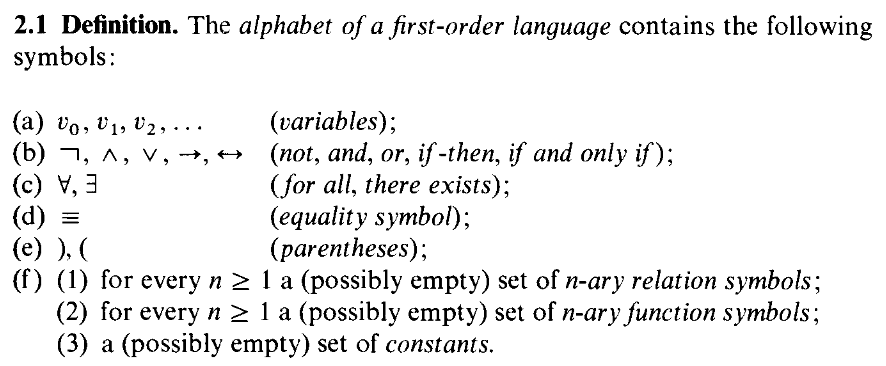
\includegraphics[scale=.5]{21}
		\end{center}

		\begin{center}
		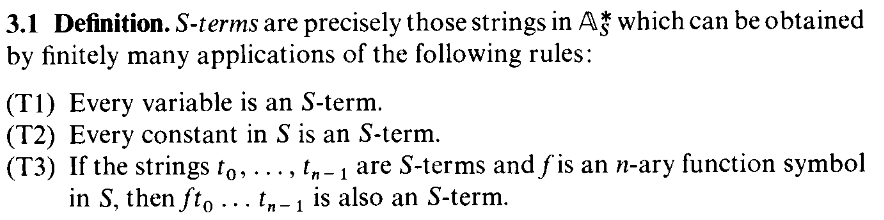
\includegraphics[scale=.5]{31}
		\end{center}

		\begin{center}
		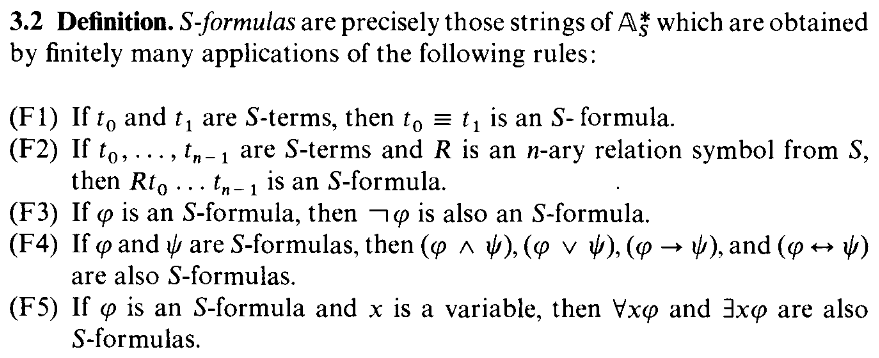
\includegraphics[scale=.5]{32}
		\end{center}

		For instance:

		\begin{center}
		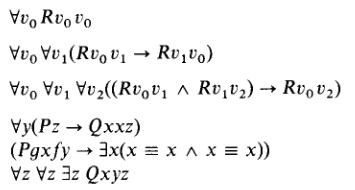
\includegraphics[scale=1]{exemplos}
		\end{center}

		\vspace{120mm}

		Conclusion | Below there's a $12 \times 26$ graph:

		\vspace{3mm}

		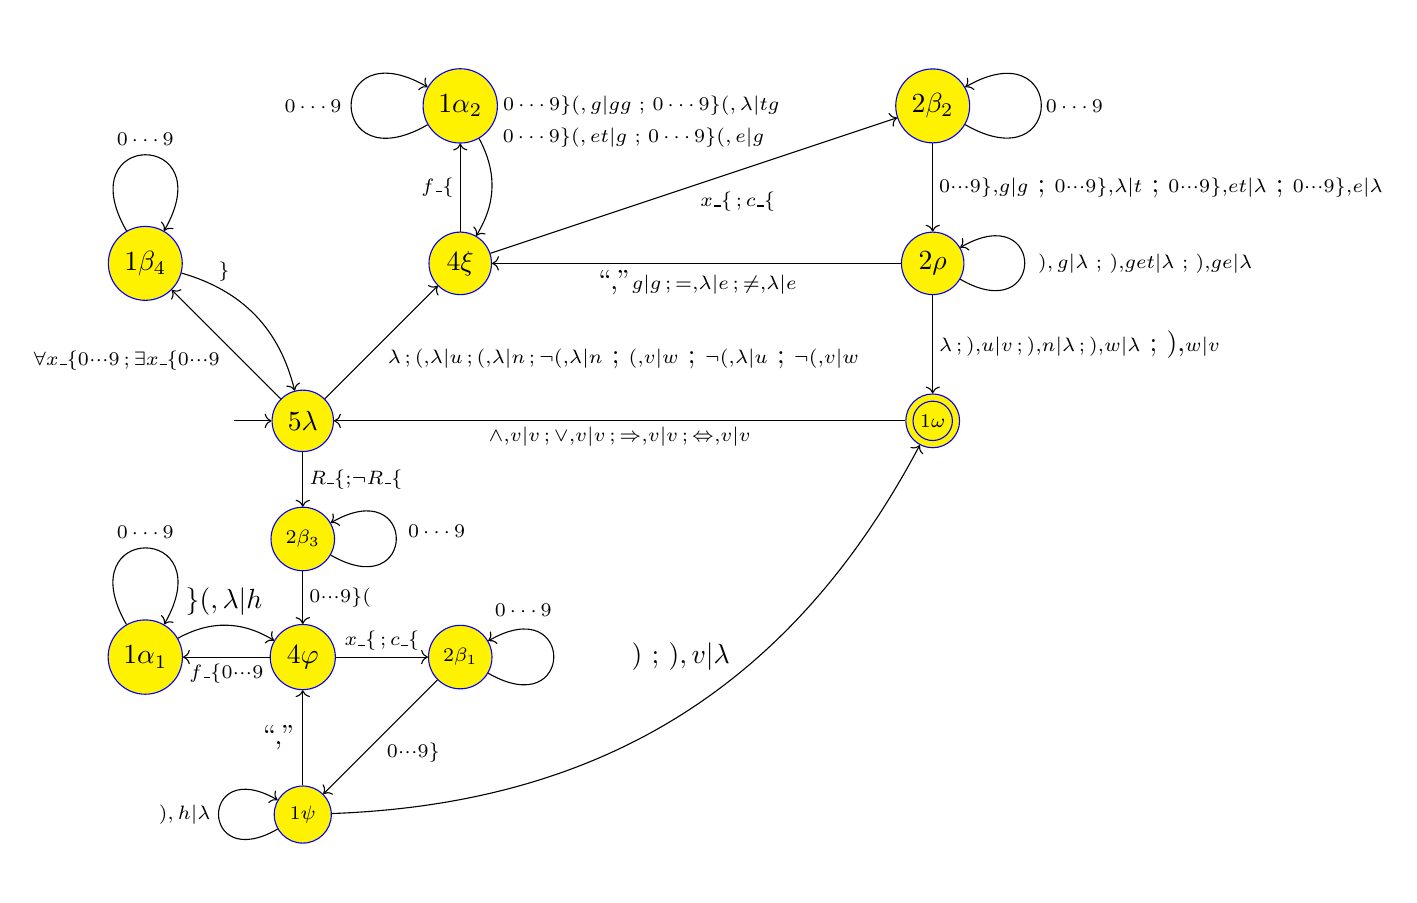
\begin{tikzpicture}
		\node (nada) at (2,0) { };
		\node[draw=blue, circle, fill=yellow] (lambda) at (3,0) {$5\lambda$};
		\node[font=\scriptsize] (lambdalinha1) at (4.7,-1.4) {$0\cdots 9$};
		\node[font=\scriptsize] (lambdalinha2) at (2, 1.9) {$\}$};
		\node (lambdalinha3) at (2, -2.3) {$\}(,\lambda|h$};
		\node[font=\scriptsize] (lambdalinha4) at (7.3, 4) {$0\cdots 9\}(,g|gg$ ; $0\cdots 9\}(,\lambda|tg$};
		\node[font=\scriptsize] (lambdalinha5) at (7.2, 3.6) {$0\cdots 9\}(,et|g$ ; $0\cdots 9\}(,e|g$};
		\node[font=\scriptsize] (lambdalinha6) at (5.8,-2.4) {$0\cdots 9$};
		\node[font=\scriptsize] (lambdalinha7) at (12.8,4) {$0\cdots 9$};
		\node[draw=blue, circle, fill=yellow] (xi) at (5,2) {$4\xi$};
		\node[draw=blue, circle, fill=yellow] (rho) at (11,2) {$2\rho$};
		\node[draw=blue, circle, fill=yellow, font=\scriptsize] (omega) at (11,0) {$1\omega$};
		\node[font=\scriptsize] (rholinha) at (13.7, 2) {$),g|\lambda$ ; ),$get|\lambda$ ; ),$ge|\lambda$};
		\draw[blue] (11,0) circle (0.25);
		\draw[->] (rho) to [in=30,out=330, loop, " "] node { } (rho);
		\node[draw=blue, circle, fill=yellow, font=\scriptsize] (c3) at (3,-1.5) {$2\beta_3$};
		\node[draw=blue, circle, fill=yellow] (varphi) at (3,-3) {$4\varphi$};
		\node[draw=blue, circle, fill=yellow] (alpha1) at (1,-3) {$1\alpha_1$};
		\node[draw=blue, circle, fill=yellow, font=\scriptsize] (c1) at (5,-3) {$2\beta_1$};
		\node (c1linha) at (7.8, -3)  {$)$ ; $),v|\lambda$};
		\node[draw=blue, circle, fill=yellow, font=\scriptsize] (psi) at (3,-5) {$1\psi$};
		\node[font=\scriptsize] (psilinha) at (1.5, -5) {$),h|\lambda$};
		\node[draw=blue, circle, fill=yellow] (c4) at (1,2) {$1\beta_4$};
		\node[draw=blue, circle, fill=yellow] (alpha2) at (5,4) {$1\alpha_2$};
		\node[draw=blue, circle, fill=yellow] (c2) at (11,4) {$2\beta_2$};
		\draw[->, font=\scriptsize] (c1) to [in=30,out=330, loop, ""] node { } (c1);
		\draw[->, font=\scriptsize] (c2) to [in=30,out=330, loop, ""] node { } (c2);
		\draw[->] (c3) to [in=30,out=330, loop, " "] node { } (c3);
		\draw[->, font=\scriptsize] (c4) to [in=60,out=120, loop, "$0\cdots 9$"] node { } (c4);
		\draw[->, font=\scriptsize] (alpha1) to [in=60,out=120, loop, "$0\cdots 9$"] node { } (alpha1);
		\draw[->, font=\scriptsize] (alpha2) to [in=150,out=210, loop, "$0\cdots 9$"] node { } (alpha2);
		\draw[->] (psi) to [in=150,out=210, loop, " "] node { } (psi);
		\draw[->, bend left] (c4) to node { } (lambda);
		\draw[->, bend left] (alpha2) to node { } (xi);
		\draw[->, bend left] (alpha1) to node { } (varphi);
		\draw[->, bend right] (psi) to node { } (omega);
		\path[commutative diagrams/.cd, every arrow, every label]
		(nada) edge node { } (lambda)
		(lambda) edge node {$R\_\{ ; \neg R\_\{$} (c3) edge node {$\forall x\_\{0\cdots 9\,;\,\exists x \_\{0\cdots 9$} (c4) edge node[swap] {$\lambda\,;\,(,\lambda|u\,;\,(,\lambda|n\,;\,\neg(,\lambda|n$ ; $(,v|w$ ; $\neg(,\lambda|u$ ; $\neg(,v|w$} (xi)
		(xi) edge node[swap] {$x\_\{\,;\,c\_\{$} (c2) edge node {$f\_\{$} (alpha2)
		(rho) edge node {``,"$g|g\,;\,=,\lambda|e\,;\,\ne,\lambda|e$} (xi) edge node {$\lambda\,;\,),u|v\,;\,),n|\lambda\,;\,),w|\lambda$ ; ),$w|v$} (omega)
		(omega) edge node {$\wedge,v|v\,;\,\vee,v|v\,;\,\Rightarrow,v|v\,;\,\Leftrightarrow,v|v$} (lambda)
		(varphi) edge node {$f\_\{0\cdots 9$} (alpha1) edge node {$x\_\{\,;\,c\_\{$} (c1)
		(c1) edge node {$0\cdots 9\}$} (psi)
		(c2) edge node {$0\cdots 9\},g|g$ ; $0\cdots 9\},\lambda|t$ ; $0\cdots 9\},et|\lambda$ ; $0\cdots 9\},e|\lambda$} (rho)
		(c3) edge node {$0\cdots 9\}($} (varphi)
		(psi) edge node {``,"} (varphi);
		\end{tikzpicture}

		\vspace{3mm}

		Let's see if exchanging $x$ by $y$ the graph looks better:

		\vspace{3mm}

		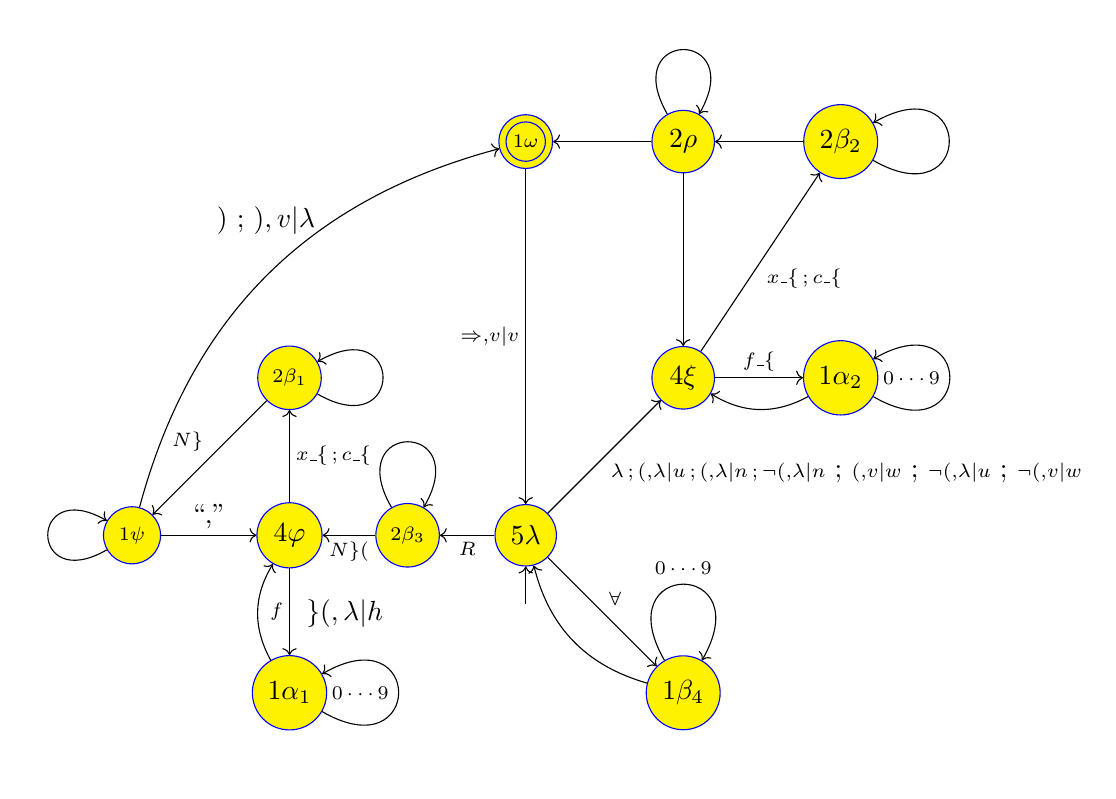
\begin{tikzpicture}
		\node (nada) at (0,2) { };
		\node[draw=blue, circle, fill=yellow] (lambda) at (0,3) {$5\lambda$};
		\node (lambdalinha3) at (-2.3, 2) {$\}(,\lambda|h$};
		\node[draw=blue, circle, fill=yellow] (xi) at (2,5) {$4\xi$};
		\node[draw=blue, circle, fill=yellow] (rho) at (2,8) {$2\rho$};
		\node[draw=blue, circle, fill=yellow, font=\scriptsize] (omega) at (0,8) {$1\omega$};
		\draw[blue] (0,8) circle (0.25);
		\draw[->] (rho) to [in=60,out=120, loop, " "] node { } (rho);
		\node[draw=blue, circle, fill=yellow, font=\scriptsize] (c3) at (-1.5,3) {$2\beta_3$};
		\node[draw=blue, circle, fill=yellow] (varphi) at (-3,3) {$4\varphi$};
		\node[draw=blue, circle, fill=yellow] (alpha1) at (-3,1) {$1\alpha_1$};
		\node[draw=blue, circle, fill=yellow, font=\scriptsize] (c1) at (-3,5) {$2\beta_1$};
		\node (c1linha) at (-3.3, 7)  {$)$ ; $),v|\lambda$};
		\node[draw=blue, circle, fill=yellow, font=\scriptsize] (psi) at (-5,3) {$1\psi$};
		\node[draw=blue, circle, fill=yellow] (c4) at (2,1) {$1\beta_4$};
		\node[draw=blue, circle, fill=yellow] (alpha2) at (4,5) {$1\alpha_2$};
		\node[draw=blue, circle, fill=yellow] (c2) at (4,8) {$2\beta_2$};
		\draw[->, font=\scriptsize] (c1) to [in=30,out=330, loop, ""] node { } (c1);
		\draw[->, font=\scriptsize] (c2) to [in=30,out=330, loop, ""] node { } (c2);
		\draw[->] (c3) to [in=60,out=120, loop, " "] node { } (c3);
		\draw[->, font=\scriptsize] (c4) to [in=60,out=120, loop, "$0\cdots 9$"] node { } (c4);
		\draw[->, font=\scriptsize] (alpha1) to [in=30,out=330, loop, "$0\cdots 9$"] node { } (alpha1);
		\draw[->, font=\scriptsize] (alpha2) to [in=30,out=330, loop, "$0\cdots 9$"] node { } (alpha2);
		\draw[->] (psi) to [in=150,out=210, loop, " "] node { } (psi);
		\draw[->, bend left] (c4) to node { } (lambda);
		\draw[->, bend left] (alpha2) to node { } (xi);
		\draw[->, bend left] (alpha1) to node { } (varphi);
		\draw[->, bend left] (psi) to node { } (omega);
		\path[commutative diagrams/.cd, every arrow, every label]
		(nada) edge node { } (lambda)
		(lambda) edge node {$R$} (c3) edge node {$\forall$} (c4) edge node[swap] {$\lambda\,;\,(,\lambda|u\,;\,(,\lambda|n\,;\,\neg(,\lambda|n$ ; $(,v|w$ ; $\neg(,\lambda|u$ ; $\neg(,v|w$} (xi)
		(xi) edge node[swap] {$x\_\{\,;\,c\_\{$} (c2) edge node {$f\_\{$} (alpha2)
		(rho) edge node { } (xi) edge node { } (omega)
		(omega) edge node[swap] {$\Rightarrow,v|v$} (lambda)
		(varphi) edge node[swap] {$f$} (alpha1) edge node[swap] {$x\_\{\,;\,c\_\{$} (c1)
		(c1) edge node[swap] {$N\}$} (psi)
		(c2) edge node { } (rho)
		(c3) edge node {$N\}($} (varphi)
		(psi) edge node {``,"} (varphi);
		\end{tikzpicture}

		\vspace{120mm}
		\Large
		\textbf{Exercise 1 | Set Theory:}
		\small
		\vspace{3mm}

		$\lambda \rightarrow F \,|\,R\,|\,GYG$ (the first and the second formulas).

		$F \rightarrow EZB\,|\, Q x\_\{N\} (F)\,|\, Q x\_\{N\} \neg(F)\,|\, Q x\_\{N\} R$, where $F$ is a formula.

		$G \rightarrow (F)\,|\,\neg(F)\,|\, GYG \,|\, (GYG)\,|\,R$ (several formulas).

		$A \rightarrow E\,|\, A, A$, where $A$ is one or more parameters.

		$B \rightarrow E\,|\,EZB$ (several equalities).

		$D \rightarrow E\,|\,(DXD)$, where $D$ is a subterm which may have parenthesis.

		$E \rightarrow T\,|\, DXD\,|\,P(E)$, where $P$ is the power set and $E$ is an Extended term.

		$T \rightarrow x\_\{N\} \,|\, c\_\{N\} \,|\, f\_\{N\}(A) \,|\, \varnothing \,|\, \{ A \}$, where $T$ is an atomic Term.

		$N \rightarrow NN \,|\, 0\,|\,1\,|\,2\,|\,3\,|\,4\,|\,5\,|\,6\,|\,7\,|\,8\,|\,9$, where $N$ is a natural number.

		$Q \rightarrow \forall\,|\,\exists\,|\,\exists\,!$, where $Q$ is a quantifier.

		$R \rightarrow ``R"\_\{N\}(A) \,|\, \neg ``R"\_\{N\}(A)$, where $R$ is a relation without parenthesis.

		$X \rightarrow \cup\,|\,\cap$ (function between terms which returns another term).

		$Y \rightarrow \wedge\,|\,\vee|\Rightarrow|\Leftrightarrow|\text{ xor}$ (operator between formulas).

		$Z \rightarrow\, =|\in|\subset|\supset|\ne\,|\notin\,|\,\cancel{\subset}\,|\,\cancel{\supset}$ (relation between terms).

		\vspace{3mm}
		\Large
		\textbf{Exercise 2 | Arithmetics:}
		\small
		\vspace{3mm}

		$\lambda \rightarrow F \,|\,R\,|\,GYG$ (the first and the second formulas).

		$F \rightarrow U_TZU_B\,|\, Q x\_\{N\} (F)\,|\, Q x\_\{N\} \neg(F)\,|\, Q x\_\{N\} R$, where $F$ is a formula.

		$G \rightarrow (F)\,|\,\neg(F)\,|\, GYG \,|\, (GYG)\,|\,R$ (several formulas).

		$A \rightarrow U_T\,|\, A, A$, where $A$ is one or more parameters.

		$B \rightarrow E\,|\,EZU_B$ (several equalities).

		$D \rightarrow E\,|\,(DXK_T)\,|\,(-DXK_T)$, where $D$ is a subterm which may have parenthesis.

		$E \rightarrow T\,|\, DXK_T$, where $E$ is an Extended term.

		$K_T \rightarrow D\,|\,(-E)$

		$U_B \rightarrow B\,|-B$

		$U_T \rightarrow E\,|-E$

		$T \rightarrow x\_\{N\} \,|\, c\_\{N\} \,|\, f\_\{N\}(A)\,|\,N$, where $T$ is an atomic Term.

		$N \rightarrow NN \,|\, 0\,|\,1\,|\,2\,|\,3\,|\,4\,|\,5\,|\,6\,|\,7\,|\,8\,|\,9$, where $N$ is a natural number.

		$Q \rightarrow \forall\,|\,\exists\,|\,\exists\,!$, where $Q$ is a quantifier.

		$R \rightarrow ``R"\_\{N\}(A) \,|\, \neg ``R"\_\{N\}(A)$, where $R$ is a relation without parenthesis.

		$X \rightarrow +\,|-\,|\,\cdot\,|\,\div$ (function between terms which returns another term).

		$Y \rightarrow \wedge\,|\,\vee|\Rightarrow|\Leftrightarrow|\text{ xor}$ (operator between formulas).

		$Z \rightarrow\, =|\ne\,|\,<\,|\,>\,|\,\le\,|\,\ge$ (relation between terms).

		\vspace{3mm}
		\Large
		\textbf{Exercise 3 | Sets of Integer Numbers | Chomsky Normal Form:}
		\small
		\vspace{3mm}

		Let the opposite of a set be $-S = \{ -x \,;\, x \in S \}$. We also may sum (and subtract, multiply, divide, order) sets.

		For instance, $A + B = \{ x + y \,;\, x \in A, y \in B \}$. Exchange ``;" by pipe too. For this language we should add:

		$G_1 \rightarrow F\,|\,R\,|\,GYG\,|\,G_1,G_1$ ; $T \rightarrow \{ E ; G_1 \} \, |\, \{ G_1 ; G_1 \}$, like $\{ (x \in \mathbb{R}) \wedge (x \notin \mathbb{Q}) \,;\, x > 0, x < 1 \}$ is an atomic Term.

		\vspace{3mm}

		$\lambda \rightarrow G_YG\,|\,E_ZB\,|\,E_ZM_B\,|M_ZB\,|M_ZM_B\,|\, Q_N P_F\,|\, Q_N N_P\,|\, Q_N R\,|\,R_UN_1 \,|\, N_RN_1$ (the first and the second formulas).

		$A \rightarrow X_ME\,|\, AV_A\,|\,D_XK_T\,|\,X_UN_4 \,|\, C_UN_4 \,|\, F_UN_1\,|\,NN \,|\, 0\,|\,1\,|\,2\,|\,3\,|\,4\,|\,5\,|\,6\,|\,7\,|\,8\,|\,9$, where $A$ is one or more parameters.

		$B \rightarrow E_ZB\,|\,E_ZM_B\,|\,D_XK_T\,|\,X_UN_4 \,|\,C_UN_4 \,|\, F_UN_1\,|\,NN \,|\, 0\,|\,1\,|\,2\,|\,3\,|\,4\,|\,5\,|\,6\,|\,7\,|\,8\,|\,9$ (several equalities).

		$D \rightarrow P_DX_K\,|\,P_MX_K\,|\,D_XK_T\,|\,X_UN_4 \,|\, C_UN_4 \,|\, F_UN_1\,|\,NN \,|\, 0\,|\,1\,|\,2\,|\,3\,|\,4\,|\,5\,|\,6\,|\,7\,|\,8\,|\,9$, where $D$ is a subterm which may have parenthesis.

		$E \rightarrow D_XK_T\,|\,X_UN_4 \,|\, C_UN_4 \,|\, F_UN_1\,|\,NN \,|\, 0\,|\,1\,|\,2\,|\,3\,|\,4\,|\,5\,|\,6\,|\,7\,|\,8\,|\,9\,|\,P_1E_2\,|\,P_1M_2$, where $E$ is an Extended term.

		$F \rightarrow E_ZB\,|\,E_ZM_B\,|M_ZB\,|M_ZM_B\,|\, Q_N P_F\,|\, Q_N N_P\,|\, Q_N R$, where $F$ is a formula.

		$G \rightarrow V_1F_2\,|\,Y_N P_F\,|\, G_YG \,|\, P_GY_G\,|\,R_UN_1 \,|\, N_RN_1$ (several formulas).

		$K_T \rightarrow P_DX_K\,|\,P_MX_K\,|\,D_XK_T\,|\,X_UN_4 \,|\, C_UN_4 \,|\, F_UN_1\,|\,NN \,|\, 0\,|\,1\,|\,2\,|\,3\,|\,4\,|\,5\,|\,6\,|\,7\,|\,8\,|\,9\,|\,P_EV_2$

		$N \rightarrow NN \,|\, 0\,|\,1\,|\,2\,|\,3\,|\,4\,|\,5\,|\,6\,|\,7\,|\,8\,|\,9$, where $N$ is a natural number.

		$Q \rightarrow \forall\,|\,\exists\,|\,Q_1Q_2$, where $Q$ is a quantifier. $Q_1 \rightarrow \exists$ ; $Q_2 \rightarrow\,!$

		$R \rightarrow R_UN_1 \,|\, N_RN_1$, where $R$ is a relation without parenthesis.

		$T \rightarrow X_UN_4 \,|\, C_UN_4 \,|\, F_UN_1\,|\,NN \,|\, 0\,|\,1\,|\,2\,|\,3\,|\,4\,|\,5\,|\,6\,|\,7\,|\,8\,|\,9\,|\,\varnothing\,|\,V_3A_4$, where $T$ is an atomic Term.

		$V_1 \rightarrow ($ ; $V_2 \rightarrow\,)$ ; $V_3 \rightarrow \{$ ; $V_4 \rightarrow\,\}$ ; $V_5 \rightarrow$ ``," ; $V_6 \rightarrow$ ``\_" ; $V_c \rightarrow c$, for a constant.	$V_f \rightarrow f$, for a function.

		$V_P \rightarrow$ ``$P$" $|$ ``$C$", where $P$ is the power set, and $C$ is the complement of a set.

		$V_R \rightarrow$ ``$R$", for a relation. $V_x \rightarrow x$, for a variable.

		$X \rightarrow +\,|-\,|\,\cdot\,|\,\div\,|\,\cup\,|\,\cap$ (function between terms which returns another term).

		$X_M \rightarrow -$ (the opposite).

		$Y \rightarrow \wedge\,|\,\vee|\Rightarrow|\Leftrightarrow|\,\oplus$ (operator between formulas). $Y_N \rightarrow\,\neg$ (not).

		$Z \rightarrow\, =|\ne\,|\,<\,|\,>\,|\,\le\,|\,\ge\,|\,\in|\subset|\supset|\notin\,|\,\cancel{\subset}\,|\,\cancel{\supset}$ (relation between terms).

		\vspace{3mm}

		\begin{tabular}{C|C|C|C|C|C|C|C}
		A_2 \rightarrow AV_2 &   E_2 \rightarrow EV_2 &   K_2 \rightarrow K_TV_2 & N_P \rightarrow Y_N P_F &  M_2 \rightarrow M_EV_2 & P_M \rightarrow V_1M_D &  R_U \rightarrow V_RU_3 & Y_G \rightarrow YG_2 \\
		A_4 \rightarrow AV_4 &	 F_U \rightarrow V_fU_3 & M_B \rightarrow X_MB & 	N_R \rightarrow Y_N R_U & P_D \rightarrow V_1D   &	P_1 \rightarrow V_PV_1 & U_3 \rightarrow V_6V_3 \\
		C_U \rightarrow V_cU_3 & F_2 \rightarrow FV_2 &   M_D \rightarrow X_MD & 	N_1 \rightarrow N_4P_A  & P_E \rightarrow V_1M_E &	Q_N \rightarrow Q_UN_4 & V_A \rightarrow V_5A \\
		D_X \rightarrow DX &     G_Y \rightarrow GY   &   M_E \rightarrow X_ME & 	N_4 \rightarrow NV_4    & P_F \rightarrow V_1F_2 & Q_x \rightarrow QV_x   &  X_K \rightarrow XK_2 \\
		E_Z \rightarrow EZ &     G_2 \rightarrow GV_2 &   M_Z \rightarrow M_EZ & 	P_A \rightarrow V_1A_2  & P_G \rightarrow V_1G   & Q_U \rightarrow Q_xU_3 &  X_U \rightarrow V_xU_3
		\end{tabular}

		\vspace{3mm}
		\Large
		\textbf{Exercise 4:}
		\normalsize
		\vspace{3mm}

		\underline{Definitions}: $a \pm b = \{ a + b, a - b \}$ ; $a \pm S = (a + S) \cup (a - S)$ ; $X \pm Y = (X + Y) \cup (X - Y)$.

		$\text{proj}(S^a, \pi^b) = \{ p(x) \in \pi^a\,;\,\forall x \in S^a, \text{ Line}(x, p(x)) \perp \pi^b \}$.

		$\langle A, B\rangle_G = A^\top \cdot G \cdot B \in \mathbb{R}$, where $A,B,G$ are matrixes. $\langle p(x), q(x)\rangle_I = \int_I p(x)\,q(x)\,\mathrm{d}x \in \mathbb{R}$.

		proj$(v, u) = \cfrac{\langle v, u \rangle}{\langle u, u \rangle} \cdot u$. $\angle(v,w) =$ arccos $\cfrac{\langle v, w\rangle}{\Vert v\Vert \cdot \Vert w \Vert} \in [0, \pi]$.

		Euler characteristic on polytopes: $$\sum_{m = 0}^{n - 1} (-1)^m \cdot V_m = 1 - (-1)^n.$$

		Below there's a finite formula: $$\Phi:\bigvee_{m = 1}^n F_m\Leftrightarrow\bigwedge_{m = 1}^n G_m.$$

		Below there are arbitrary extensions: $$B = \bigcup_{n \in \mathbb{N}} A_n\,;\,C = \bigcap_{\lambda \in ]0,1[} A_\lambda\,;\,\Phi:\bigvee_{n \in \mathbb{N}} F_n\Leftrightarrow\bigwedge_{\lambda \in ]0,1[} G_\lambda.$$

		\begin{myenum}
		\item The goal here is to group everything: scalar number element, set (line, plane, polygon, polyhedron, polytope, circle, sphere, ball, cylinder, cone), function, tensor, vector, point, differential form, monomial, polynomial, algebraic fraction, matrix, infinity and so on.
		\item Separate elements from sets. term $X$ term ; $X \rightarrow M_P\,|\,\cdot\,|\,\div$ ; term $Z$ term ; $M_P \rightarrow +\,|-$ ;

		$Z \rightarrow\,=\,|\,\ne\,|\,<\,|\,>\,|\,\le\,|\,\ge\,|\,\propto$. set $X_S$ set ; $X_S \rightarrow X\,|\,\cup\,|\,\cap\,|\,\pm\,|\,\times$ ; set $Z_S$ set ;

		$Z_S \rightarrow Z\,|\,\in\,|\,\notin\,|\,\subset\,|\,\supset\,|\,\pitchfork\,|\,\cancel{\subset}\,|\,\cancel{\supset}$, for transversal sets. term $Z_{TS}$ set ; $Z_{TS} \rightarrow\,\in\,|\,\notin$ ; set $Z_{ST}$ term ; $Z_{ST} \rightarrow\,\ni\,|\,\cancel{\ni}$ ; set $\rightarrow$ term $\pm$ set ; set $\rightarrow$ term $\pm$ term ; set $\rightarrow$ term $X$ set ; set $\rightarrow$ set $X$ term.
		\item $S_E \rightarrow S\,|\,S_DX_SK_S\,|\,K_T X K_S\,|\,U_S X H$ ; $S_D \rightarrow S_E\,|\,(S_DX_SK_S)\,|\,(-S_DX_SK_S)$, for linear combination of scalars and sets. Also for non Abelian $x \cdot N \ne N \cdot x$ and Cartesian product.
		\item $U_S \rightarrow S_E\,| -S_E$ ; $K_S \rightarrow S_E\,|\,(-S_E)$.
		\item $E \rightarrow \gcd(U_T, A)\,|\,$lcm$(U_T, A)$, for greatest common divisor and least common multiple.
		\item $F \rightarrow U_TX_DU_T$ ; $X_D \rightarrow V_9\,|\,\nmid$ ; $V_9 \rightarrow ``|"$, for $a$ does [not] divide $b$.
		\item $X_T \rightarrow /\,|\,\wedge$ ; $E \rightarrow$ cfrac$\{E\}\{E\}$, for fractions and $c^x$ ; $\varphi\wedge\varphi$; set $\wedge$ set; $p(x)\wedge K_N$ ; matrix $\wedge$ matrix;

		group\_element $W \wedge\,K_N$ ; $\infty\wedge K_N$.
		\item $T \rightarrow N.N\,|\,N.(N)\,|\,N.N(N)$, for floating point. $U_N \rightarrow N\,|-N$ ; $K_N \rightarrow N\,|\,(-N)$.
		\item $H \rightarrow T\,|\,(U_T)$ ; $E \rightarrow X_E\,H\,|\text{ sqrt }H\,|\,\text{sqrt}[U_T]\,H\,|\,\exp H\,|\text{ argtanh }H\,|\,\text{ord }K_T$, for order of an element.
		\item $X_E \rightarrow \log\,|\,\ln\,|\,\log\_\{U_T\}\,|\,\sin\,|\,\cos\,|\,\tan\,|\,\sec\,|\,\cot\,|\text{ cossec}$ ; $E \rightarrow X_E\wedge K_N\,H$.
		\item Define $H_S, H_\varphi, H_V, H_\omega, H_J, H_\alpha, H_C, H_N$.
		\item $E \rightarrow \arcsin H\,|\,\arccos H\,|\,\arctan H\,|\,\sinh H\,|\,\cosh H\,|\,\tanh H\,|\,\coth H\,|\,\text{argsinh }H\,|\,\text{argcosh }H$.
		\item $E \rightarrow \lfloor U_T \rfloor\,|\, \lceil U_T \rceil$, for floor and ceiling. $T \rightarrow i\,|\,j\,|\,k$, for complex unity and quaternions.
		\item $E \rightarrow E!\,|\,\Gamma(U_T)\,|$ binom$(U_T, U_T)$, for factorial and Newton binomial. Do the same for finite sequences and permutations with[out] repetitions.
		\item $E \rightarrow V_9U_TV_9\,|\,\Re\text{e}\,H\,|\,\Im\text{m}\,H\,|$ conjugate$(U_T)\,|$ arg $H$, for absolute value, argument, real and imaginary part.
		\item Use functions without parameters: $\varphi \rightarrow f\_\{N\}\,|\,\text{Id };\,X_\varphi \rightarrow X\,|\,X_T\,|\,\circ$ ; $\varphi X_\varphi \varphi$ ; $\varphi Z \varphi$.
		\item Define $\varphi_D, \varphi_E, K_\varphi, U_\varphi, H_\varphi$, for linear combination of scalars and $\varphi$s.
		\item $\varphi_E \rightarrow K_\varphi|_\_{K_S}$, for restriction of domain. Everything may be parameter for $f_N, R_N, \varphi$.
		\item $S_E \rightarrow$ Dom $H_\varphi\,|$ Range $H_\varphi\,|$ Im $H_\varphi\,|$ Ker $H_\varphi\,|$ $\Gamma\,H_\varphi\,|$ supp $H_\varphi$, for image, kernel, graphic and support.
		\item $E \rightarrow \delta(F)\,|\,\delta(R)\,|\,\delta(GYG)$, for $\delta(c = 0)$. $L \rightarrow T\,|\,\infty$ and define $L_D, L_E, K_L, U_L, H_L$.
		\item $V \rightarrow (U_T, U_T)$, for an ordered pair. Separate scalars from vectors. vector $Z_V$ vector ; $Z_V \rightarrow\,=\,|\,\ne$.
		\item $X_V \rightarrow M_P\,|\,\times$ ; $V_E \rightarrow V\,|\,V_D X_V K_V\,|\,K_T\cdot K_V$ ; $V_D \rightarrow V_E\,|\,(V_D X_V K_V)\,|\,(-V_D X_V K_V)$, for linear combination of scalars and vectors. Also for Euclidean cross product.
		\item $U_V \rightarrow V_E\,| -V_E$ ; $K_V \rightarrow V_E\,|\,(-V_E)$. $E \rightarrow \langle U_V, U_V \rangle$, for Euclidean inner product.
		\item $V_E \rightarrow \nabla H\,|\,\nabla \times K_V$, for gradient and curl. $E \rightarrow \langle \nabla, U_V \rangle$, for divergence.
		\item $\varphi \rightarrow$ Id$(S_E)$ ; $F \rightarrow U_V=U_V\,|\,U_V\ne U_V\,|\,U_V Z_{TS} S_E$, where $S_E$ is an extended set.
		\item $L_E \rightarrow$ dim $K_S\,|$ codim $K_S\,|$ $\inf K_S\,|\,\sup K_S\,|\,\text{inf}\_\{x\_\{N\} \in S_E\}\,H\,|\,\text{sup}\_\{x\_\{N\} \in S_E\}\,H$.
		\item So we related vector and set. And all the possibilities are binom$(11,2)\cdot 2 = 110$ ($g$ for tensor, $W$ for group element which is not a number, $2 = X + Z$):

		\begin{tabular}{C|C|C|C|C|C|C|C|C|C|C|C|C|C}
		 TS  &		 T\varphi &  S\varphi &		 TV &  SV &  \varphi V &		 T\omega &  S\omega &  \varphi\omega &  V\omega &		 TJ	&		 SJ      &  \varphi J    &  VJ      \\
		 \omega J &	 T\alpha &  S\alpha &  \varphi\alpha &  V\alpha &  \omega\alpha &  J\alpha & TC	&
		 SC      &  \varphi C     &  VC      &  \omega C     &  JC      &  \alpha C \\
		 TW	&  SW      &  \varphi W     &  VW      &  \omega W   &		 JW     &  \alpha W &  CW &  TL	&  SL      &  \varphi L     &  VL      &  \omega L    &  JL     \\
		 \alpha L &  CL &	 WL &	 Tg	&  Sg      &  \varphi g     &  Vg      &  \omega g    &  Jg     &  \alpha g &  Cg & Wg & Lg
		\end{tabular}
		\item $F \rightarrow$ open$(S_E)$, closed$(S_E)$, clopen$(S_E)$. $E \rightarrow \min K_S\,|\,\max K_S\,|\,\text{card }K_S$, for finite cardinality.
		\item $S_E \rightarrow K_S\,^\perp\,|\,\partial K_S\,|$ interior$(S_E)\,|$, closure$(S_E)\,|$  completion$(S_E)\,|\,\text{Frac }K_S\,|\,M\_\{N\times N\} K_S\,|\,\text{extended}(U_S)$.

		$S_E \rightarrow H_S\wedge N$, for Euclidean orthogonal complement, border, set (field) of fractions, set (ring) of matrixes $N\times N$,	set $\cup\,\{\infty, -\infty\}$ and Cartesian product of $n$ copies of set.
		\item $S_E \rightarrow V_bM_1, M_1V_b$ ; $V_b \rightarrow ``["\,|\,``]"$ ; $M_1 \rightarrow U_T\,|\,\infty\,|-\infty$, for an interval.
		\item $V \rightarrow (A)$, for an element of $\mathbb{R}^n$. $V \rightarrow e\_\{N\}$, for canonical basis vector.
		\item $L_E \rightarrow$ dist$(U_V, U_V)$ ; $E \rightarrow \angle(U_V,U_V)$, for Euclidean metric and angle.
		\item $V_E \rightarrow$ proj$(U_V, U_V)$. $L_E \rightarrow V_9V_9U_VV_9V_9$, for Euclidean norm.
		\item $L_E \rightarrow$ dist$(S_E, S_E)$ ; $E \rightarrow \angle(S_E,S_E)$, for Euclidean metric and angle between sets.
		\item $S_E \rightarrow$ proj$(S_E, S_E)$, for Euclideanly orthogonal projection of set into another set.
		\item $F \rightarrow U_V \perp U_V\,|\,U_V \parallel U_V$, for Euclidean orthogonality and parallelism.
		\item $F \rightarrow S_E \perp S_E\,|\,S_E \parallel S_E$, for Euclidean orthogonality and parallelism between sets.
		\item $F \rightarrow S_E \sim S_E\,|\,S_E \cong S_E$, for similar and congruent sets.
		\item $X_\sigma \rightarrow ``S"$ ; $S_E \rightarrow X_\sigma\wedge N(U_V, U_T)\,|\,X_\sigma\wedge N(U_C, U_T)\,|\,X_\sigma\wedge N(U_\varphi, U_T)$, for Euclidean circle and sphere.
		\item $X_\sigma \rightarrow ``S"\_\{N\}$, for sphere by $n$th metric or by $n$th norm.
		\item $X_B \rightarrow ``B"$ ; $S_E \rightarrow X_B\wedge N(U_V, U_T)\,|\,X_B\wedge N(U_C, U_T)\,|\,X_B\wedge N(U_\varphi, U_T)$, for Euclidean ball.
		\item $X_B \rightarrow ``B"\_\{N\}$, for ball by $n$th metric or by $n$th norm.
		\item $S_E \rightarrow \langle A_3 \rangle$ ; $A_3 \rightarrow A_3, A_3\,|\,U_V$, for the vectorial space generated by $n$ vectors.
		\item $S_E \rightarrow U_V M_P S_E$, for the translation of one vectorial space by one vector.
		\item $S_E \rightarrow$ Line$(U_V, U_V)$, for the line through two distinct points $v_0 + \langle v_1 - v_0 \rangle$. Geodesics.
		\item $S_E \rightarrow \pi\wedge N(U_V, U_V, A_3)$, for the plane$^n$ through $3$ or more general points $v_0 + \langle v_1 - v_0, v_2 - v_0, \cdots, v_n - v_0 \rangle$.
		\item $S_E \rightarrow$ Cylinder$(U_S, U_V)$, for $\{w + t d\,;\,w \in S \subset \pi^2, d \in \pi^3 - \pi^2\}$.
		\item $S_E \rightarrow$ Cone$(U_S, U_V)$, for $\{v + t (w - v)\,;\,w \in S \subset \pi^2, v \in \pi^3 - \pi^2\}$.
		\item $S_E \rightarrow$ Polygon$(U_V, U_V, A_3)$, for $3$ or more distinct points $\subset \pi^2, e_{0,1} = \{v_0 + t(v_1 - v_0), t \in [0,1]\}$

		$\Rightarrow x = \cfrac{n(n-3)}{2}$ empty intersections of line segments. Adjacent edges intersect at $n$ vertices. Diagonals intersect at $x$ interior points.
		\item $S_E \rightarrow$ Polyhedron$(U_V, U_V, U_V, A_3)$, for $4$ or more distinct points $\subset \pi^3, V_0 - V_1 + V_2 = 2$.
		\item $S_E \rightarrow$ Polytope$(U_V, U_V, U_V, U_V, A_3)$, for $5$ or more distinct points $\subset \pi^n, n \ge 4$, Euler holds.
		\item $L_E \rightarrow V_9V_9U_VV_9V_9\_\{N\}$, for $n$th norm. $L_E \rightarrow$ dist$\_\{N\}(U_V, U_V)$, for $n$th metric.
		\item $E \rightarrow \langle U_V, U_V\rangle\_g\,|\, g(U_V, U_V)$, for $n$th inner product. Is $g$ our first tensor?
		\item $V_E \rightarrow$ proj$\_\{N\}(U_V, U_V)$, for $n$th projection of one vector onto another.
		\item $S_E \rightarrow$ proj$\_\{N\}(S_E, S_E)$, for $n$th projection of one set into another. $V_S \rightarrow \Sigma\,|\,\Pi$ ; $V_L \rightarrow \lambda\,|\,V_LV_L\,|\,'$.
		\item $L_E \rightarrow V_S\_\{x\_\{N\} \in S_E\} H$, for sum or product over one set. If $S_E$ is countable, then this is one series.
		\item $L_E \rightarrow V_S\_\{x\_\{N\} = U_T\}\wedge\{U_T\} H$, for sum and product from $\{n = t_0\}$ to $t$.
		\item $\varphi_E \rightarrow fV_L\_\{N\}$ ; $L_E \rightarrow fV_L\_\{N\}(A)$, for mono derivative. That function may assume $\infty$ values.
		\item $\varphi_E \rightarrow fV_LM_P\_\{N\}$, for lateral mono derivative without parameter. That function may assume $\infty$ values.
		\item $\varphi_E \rightarrow N_2$ ; $E \rightarrow N_2(A)$ ; $N_2 \rightarrow f\_\{N\}\wedge(N)\,|\,f\_\{N\}\wedge[U_N]$, for $(n)$th derivative or $[-n]$th iteration of $f$.
		\item $\varphi_E \rightarrow P_2 H_\varphi$ ; $E \rightarrow P_2 H$ ; $P_2 \rightarrow P_2P_2\,|\,\partial/(\partial x\_\{N\})$, for partial derivative.
		\item $\varphi_E \rightarrow P_3 H_\varphi$ ; $E \rightarrow P_3 H$ ; $P_3 \rightarrow \partial\wedge N/(P_4)$ ; $P_4 \rightarrow \partial x\_\{N\}\,|\,\partial x\_\{N\}\wedge N\,|\,P_4 P_4$, for $\partial^3/(\partial x^2 \partial y)$.
		\item $E \rightarrow V_7E_3D_5$ ; $E_3 \rightarrow V_7E_3D_5\,|\,H$ ; $V_7 \rightarrow \int$ ; $D_5 \rightarrow \mathrm{d}x\_\{N\}$, for indefinite integral.
		\item $V_E \rightarrow V_7E_5D_5$ ; $E_5 \rightarrow V_7E_5D_5\,|\,K_V$, for vectorial indefinite integral.
		\item $V_I \rightarrow V_7\,|\,\overline{\int}\,|\,\underline{\int}$ ; $L_E \rightarrow V_I\_\{V_bM_1,M_1V_b\} E_4 D_5$ ; $E_4 \rightarrow V_I\_\{V_bM_1,M_1V_b\}E_4D_5\,|\,H$, for definite integral, superior integral and inferior integral.
		\item $V_E \rightarrow V_I\_\{V_bM_1,M_1V_b\} E_6 D_5$ ; $E_6 \rightarrow V_I\_\{V_bM_1,M_1V_b\}E_6D_5\,|\,K_V$, for vectorial definite, vectorial superior and vectorial inferior integral. Each cohordinate may be $\infty$.
		\item Riemann-integrable $\varphi(x)$. Lebesgue spaces $L^p$.
		\item $X_\omega \rightarrow M_P\,|\,\wedge$ ; $\omega_E \rightarrow \omega\,|\,\omega_DX_\omega K_\omega \,|\,K_T\cdot K_\omega$ ; $\omega_D \rightarrow \omega_E\,|\,(\omega_DX_\omega K_\omega)\,|\,(-\omega_DX_\omega K_\omega)$, for wedge product and linear combination of scalars and $\omega$s.
		\item $U_\omega \rightarrow \omega_E\,| -\omega_E$ ; $K_\omega \rightarrow \omega_E\,|\,(-\omega_E)$. $V_8 \rightarrow \mathrm{d}\,|\,V_8V_8$ ; $\omega_E \rightarrow V_8x\_\{N\}\,|\,V_8K_3$, for differential of $\omega$.
		\item $E \rightarrow V_7\_K_S\,K_4$, for integral over set $K_S$ of one differential form $\omega$.
		\item Same for the entire language of vectorial analysis. [SPIVAK, Michael. Calculus on Manifolds].
		\item $J_E \rightarrow J\,|\,J_D X_J K_J$ ; $J_D \rightarrow J_E\,|\,(J_DX_J K_J)\,|\,(-J_DX_J K_J)$, for linear combination of scalars and monomials.
		\item $U_J \rightarrow J_E\,| -J_E$ ; $K_J \rightarrow J\,|\,(U_J)$ ; $X_J \rightarrow M_P\,|\,\cdot\,|\,\div$.
		\item $J \rightarrow c\_\{N\} J_M\,|\,N J_M$ ; $J_M \rightarrow x\_\{N\}\wedge N\,|\,J_M\cdot J_M$, for monic monomials.
		\item $E \rightarrow \deg K_J$ ; $J \rightarrow U_J \div K_J\,|\,\gcd(U_J, U_J)\,|\,\text{lcm}(U_J, U_J)$, for operations with polynomials.
		\item $L_E \rightarrow$ dist$(\varphi_E, \varphi_E)$ ; $E \rightarrow \angle(\varphi_E,\varphi_E)\,|\,\langle \varphi_E, \varphi_E \rangle$, for Euclidean metric, inner product and angle between functions. $L_E \rightarrow V_9V_9U_\varphi V_9V_9$, for Euclidean function norm.
		\item $\alpha \rightarrow J_E/K_J\,|\,J_E\,|\,\text{cfrac}\{U_J\}\{U_J\}$ ; $X_\alpha \rightarrow X_J\,|\,/$, for algebraic fractions with[out] denominator. $\alpha\wedge N$.
		\item $U_\alpha \rightarrow \alpha_E\,| -\alpha_E$ ; $K_\alpha \rightarrow \alpha_E\,|\,(-\alpha_E)$. Polynomials and algebraic fractions as $\varphi$ or $\varphi(x)$.
		\item $\alpha_E \rightarrow \alpha_D X_\alpha K_\alpha$ ; $\alpha_D \rightarrow \alpha\,|\,(\alpha_E)\,|\,(\alpha_D X_\alpha K_\alpha)\,|\,(-\alpha_D X_\alpha K_\alpha)$ ; $K_\alpha \rightarrow \alpha_D\,|\,(-\alpha_E)$, for operations between $\alpha$s.
		\item $F \rightarrow U_T \equiv U_T (\text{mod }H)$, for modulo scalar. $S_E \rightarrow [U_T]\_\{U_T\}$, for modulo scalar equivalence class.
		\item $S_E \rightarrow S_E / K_S$, for set over set. $S_E \rightarrow S_E / R\_\{N\} (A)$, for set over relation.
		\item $F \rightarrow U_J \equiv U_J (\text{mod }K_J)$, for modulo polynomial. $W \rightarrow e\_\{U_S\}$, for group identity.
		\item $S_E \rightarrow [U_J]\_\{U_J\}$, for modulo polynomial equivalence class.
		\item $S_E \rightarrow [U_T]\_\{R\_\{N\}\}$, for relation between scalars equivalence class.
		\item $S_E \rightarrow [U_J]\_\{R\_\{N\}\}$, for relation between polynomials equivalence class. Same for $U_\varphi, U_V, U_\omega, U_\alpha, U_C, U_N$.
		\item $S_E \rightarrow K_S[A_1]$ ; $A_1 \rightarrow A_1, A_1\,|\,x\_\{N\}$, for the set (ring) of polynomials $\mathbb{Z}[x,y]$.
		\item $S_E \rightarrow U_J \cdot K_S$, for polynomial times set. $F \rightarrow U_S \lhd K_S$, for normal subgroup.
		\item What about this notation? $C \rightarrow (A)\_\{N \times N\}$, for matrix.

		Example: $(a_{11}, a_{12}, a_{13}, a_{21}, a_{22}, a_{23})_{2 \times 3}$ is one matrix.
		\item $X_C \rightarrow M_P\,|\,\cdot$ ; $C_E \rightarrow C\,|\,C_DX_C K_C\,|\,K_T\cdot K_C$ ; $C_D \rightarrow C_E\,|\,(C_DX_C K_C)\,|\,(-C_D X_C K_C)$, for multiplying matrix by matrix and linear combination of scalars and matrixes.
		\item $U_C \rightarrow C_E\,| -C_E$ ; $K_C \rightarrow C_E\,|\,(-C_E)$. $V_E \rightarrow C_E\cdot K_V$, for multiplying matrix by vector.
		\item $C_E \rightarrow K_C\,^\top\,|\,K_C\wedge K_N\,|\,\det K_C\,|\,\text{rank }K_C\,|\,\text{tr }K_C\,|\,\exp K_C\,|\,\ln K_C\,|\,\ker K_C$, for transpose, inverse, $n$th power,

		determinant, rank, trace, exponential, logarithm and kernel of matrix.
		\item $C_E \rightarrow V_8H\,|\,V_8f\_\{N\}$, for differential of scalar. $C_E \rightarrow V_8K_V$, for differential of vector.
		\item $L_E \rightarrow$ dist$(C_E, C_E)$ ; $E \rightarrow \angle(C_E,C_E)\,|\,\langle C_E, C_E \rangle$, for Euclidean metric, inner product and angle between matrixes. $L_E \rightarrow V_9V_9U_CV_9V_9$, for Euclidean matrix norm.
		\item $V_{10} \rightarrow \lim\,|\,\liminf\,|\,\limsup$ ; $L_E \rightarrow V_{10}[x\_\{N\} \rightarrow U_L] H_\varphi$, for limit, inferior limit, superior limit.
		\item $L_E \rightarrow V_{10}[x\_\{N\} \rightarrow U_T M_P] H_\varphi$, for lateral limit. Use also $\varphi(x+)$. Maybe $A \rightarrow AM_P$ solves everything.
		\item $V_{10} \rightarrow \text{lim}\_\{N\}$, for limit by $n$th metric or $n$th norm. Limit of vector. $\underset{(x,y) \rightarrow (a_+,b_+)}{\text{lim}_2} \sin xy = 1$.
		\item Sequence of real numbers $x_n \in \mathbb{R}^\omega$. Limit of $x_n$ while $n \rightarrow +\infty$. Limit $= c \in \mathbb{R}$ or $+\infty$ or $-\infty$. Limit $\in \varnothing$.

		$v \in \mathbb{R}^{\{1,2\}} \Rightarrow v(1) = v_1 \in \mathbb{R}, v(2) = v_2 \in \mathbb{R}$. $v$ is also one function.

		$v \in \mathbb{R}^\omega \Rightarrow s_n = v_1 + \cdots + v_n$ ; object: $(s_n)_{n \in \mathbb{N}}$ ; $\lim s_n = \underset{n \in \mathbb{N}}{\sum} v_n \in \text{extended}(\mathbb{R})$.
		\item Space $v \in \mathbb{R}^{]0,1[} \Rightarrow$ object: $(v_\lambda)_{\lambda \in ]0,1[}$. Define the sets $\varphi \in C^0, C^1, \cdots, C^\infty$.
		\item Sequence of functions $\varphi_n \in (\text{Range}^\text{Dom})^\omega$. Limit of $\varphi_n$ while $n \rightarrow +\infty$. Limit $= \varphi \in \mathbb{R}^{]0,1[}$ or $\text{extended}(\mathbb{R})^{]0,1[}$. Limit $\in \varnothing$. Several convergences: pointwise and uniform.

		$f \in (\text{Range}^\text{Dom})^{\{1,2\}} \Rightarrow f(1) = f_1 \in C(]0,1[, \mathbb{R}), f(2) = f_2 \in C(]0,1[, \mathbb{R})$.

		$f \in (\text{Range}^\text{Dom})^\omega \Rightarrow$ object: $(f_n)_{n \in \mathbb{N}}$ ; $\lim f_n = f \in C(]0,1[, \text{extended}(\mathbb{R}))$.

		$\sigma_n = f_1 + \cdots + f_n \Rightarrow$ object: $(\sigma_n)_{n \in \mathbb{N}}$ ; $\lim \sigma_n = \underset{n \in \mathbb{N}}{\sum} f_n = \sigma \in C(]0,1[, \text{extended}(\mathbb{R}))$.

		$f \in (\text{Range}^\text{Dom})^{]0,1[} \Rightarrow$ object: $(f_\lambda)_{\lambda \in ]0,1[}$.
		\item Family of sets. Infinite cardinalities $\aleph_k$. $A \in P(\mathbb{N})^\omega \Rightarrow A(1) = A_1 \subset \mathbb{N}, A(2) = A_2 \subset \mathbb{N}$.
		\item Sequence of vectors. $v \in (\mathbb{R}^n)^{\{1,2\}} \Rightarrow v(1) = v_1 \in \mathbb{R}^n, v(2) = v_2 \in \mathbb{R}^n$. $v$ is also one function.

		$v \in (\mathbb{R}^n)^\omega \Rightarrow s_n = v_1 + \cdots + v_n$ ; object: $(s_n)_{n \in \mathbb{N}}$ ; $\lim s_n = \underset{n \in \mathbb{N}}{\sum} v_n \in \text{extended}(\mathbb{R}^n)$.
		\item Sequence of: polynomials, $\alpha$s, matrixes, infinities and tensors.
		\item tensor $\otimes$ tensor; Differential form as tensor. $n$th differential of $f$ at point $p$ applied to $n$ vectors. Pullback.
		\item Handle three dots: $DXK_TX\cdots$, $GYGY\cdots$, $EZU_BZ\cdots$, $A, A, \cdots$, $\delta$, linear combination $+ \cdots$,

		$U_V=U_V=\cdots$, $U_V\perp U_V\perp\cdots$, $S \sim S \sim\cdots$, $D_6\cdot K_6\cdot\,\cdots$.
		\item List of types: formula, natural, integer, rational, irrational[algebrical], irrational[S\_transcendent],

		irrational[T\_transcendent], irrational[Liouville\_transcendent], real, complex, function, relation, set[real],

		interval[real], vector[real], sequence[real], sequence[set], family[integer], sequence[formula], family[formula], polynomial[real], algebraic\_fraction[integer], matrix[real], differential\_form, monic\_monomial, group\_element, extended[real], extended[vector[real]], tensor, quaternion.

		$f = \lim$ function[$A$:interval, $B$:real] is function[$A$:interval, $C$:extended[real]].
		\item $c, x$ is type, for element. $\mathbb{Z}$ is set[int]. $\mathbb{Z}_2$ is set[set[int]], for $\{2\mathbb{Z}, 2\mathbb{Z} + 1 \}$.
		\item $v \in M^n,\,T_pM,\,TM$; $X: M \rightarrow TM$. Fibrations. $\omega \in \Lambda^k(\mathbb{R}^n) \subset T^k_\ell(\mathbb{R}^n)$.
		\item $f$ is function[$A$:type, $B$:type], for types of domain $=A$ and range $=B$. For instance, for each polynomial $p$, one vector $v = f(p)$ ; $f$ is function[$A$:polynomial, $B$:vector] ; $f(a_0 + \cdots + a_n x^n) = (a_0, \cdots, a_n)$.
		\item Relation[type, type] is not needed, if every object has its own type.
		\item Partial differential equation: $u_{xx} + u_{yy} + u_x + u_y = u$.
		\item $n$-ary conjunction and disjunction of formulas.
		\item Units$(U_S)$, Irred$(U_S)$ for primes. Center, centralizer, normalizer, stabilizer, orbit, conjugation class...
		\item Check for ambiguity errors.
		\end{myenum}

		\vspace{3mm}

Portuguese Main Video on \href{https://www.youtube.com/watch?v=OUaltUyhTSM}{\color{blue}\underline{YouTube}}.

\end{document}
